\documentclass[12pt]{article}
 \usepackage{graphicx} 
\usepackage{multirow}
\usepackage{listings}
\usepackage{pythonhighlight}
\usepackage{todonotes}
\begin{document}
\title{Exploration and Presentation - Assignment 3}
\maketitle
\author{
  benjamin kongshaug
  \texttt{cph-bk131@cphbusiness.dk}

}
\author{
  Amanda Hansen
  \texttt{cph-ah433@cphbusiness.dk}

}
\author{
  Amalie Landt
  \texttt{cph-sl307@cphbusiness.dk}

}
\thispagestyle{empty}
\pagebreak

\setcounter{secnumdepth}{4}
\tableofcontents

\pagebreak

\section{Task 1}

\subsection{Find a point in your program that can be optimized (for speed), for example by using a profiler}

Før optimering tager programmet: Time elapsed (millisec): 389 \\ \\
Først og fremmest kan vi se 83 procent af tiden befinder programmet sig i metoden tallychars og at det er her vi skal optimere \\ \\
Sekundært ser vi en ligelig fordeling på 33,3 procent af tiden brugt på at lægge input i hashMap og på at læse fra input reader filen \\ \\
Vi kan optimere ved at finde en alternativ måde at indlæse fra filen og ved at gemme mængden af hver bogstav på en mere effektiv måde

\begin{figure}[h!]
\begin{center}
\caption{Output fra profiler}
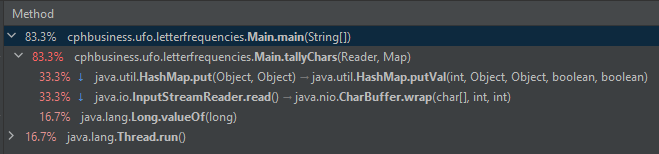
\includegraphics[width=9cm,height=5cm]{før_optimering.PNG}
\label{fig:cclogo}
\end{center}
\label{fig:firstFigureLabel}
\end{figure}

\subsection{A hypothesis of what causes the problem}
Reader reader = new FileReader(fileName);
En reader læser data fra en fil, en linje af gangen når man bruger reader.read() hvilket ikke er særlig effektivt når man har af gøre med en stor fil 

\subsection{A changed program with better performance}
ved at anvende en BufferedInputStream istedet for en reader kan vi gøre indlæsningen af dataen hurtigere, da vores .read metode tager mod data fra bufferen istedet for filen og det er hurtigere at indlæse data fra en buffer. \\ \\

Vi forbedre programmet ved at anvende en Buffered input stream som illustret nedenfor:

\begin{figure}[h!]
\begin{center}
\caption{Output fra profiler}
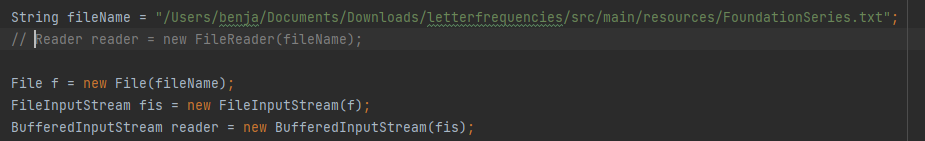
\includegraphics[width=9cm,height=5cm]{forandring.PNG}
\label{fig:cclogo}
\end{center}
\label{fig:firstFigureLabel}
\end{figure}


\subsection{Make a measurement of the point to optimize, for example by running a number of times, and calculating the mean and standard deviation (see the paper from Sestoft)}

Tid for metoden at køre før optimering i millisec over 100 kørsler :

\begin{equation}
[394, 394, 394, 394, 394, 394, 395, 395, 395, 395, 397, 397, 397, 397, 397, 397, 397, 397, 397, 397, 397, 397, 397, 398, 398, 398, 398, 398, 398, 398, 398, 398, 398, 398, 398, 398, 398, 398, 398, 398, 399, 399, 399, 399, 399, 399, 399, 399, 399, 399, 399, 399, 399, 399, 399, 399, 399, 399, 399, 399, 399, 399, 399, 402, 402, 402, 402, 402, 402, 405, 405, 405, 405, 405, 405, 405, 405, 405, 405, 405, 405, 405, 405, 405, 405, 405, 405, 405, 405, 405, 405, 405, 405, 406, 406, 406, 406, 407, 407, 407]
\end{equation}
Tid for metoden at køre efter optimering i millisec over 100 kørsler:

\begin{equation}
[202, 202, 202, 202, 202, 202, 202, 202, 202, 202, 202, 202, 202, 202, 202, 202, 202, 202, 202, 202, 202, 202, 202, 202, 202, 202, 202, 202, 202, 202, 202, 202, 202, 202, 202, 202, 202, 202, 202, 202, 202, 202, 202, 202, 202, 202, 202, 202, 202, 202, 202, 202, 203, 203, 203, 203, 203, 203, 203, 203, 203, 203, 203, 203, 203, 203, 203, 203, 203, 203, 203, 203, 203, 203, 203, 203, 203, 203, 203, 203, 203, 203, 203, 203, 203, 203, 203, 203, 203, 203, 203, 203, 203, 203, 203, 203, 203, 203, 203, 203]
\end{equation}

\begin{figure}[h!]
\begin{center}
\caption{Output fra profiler}
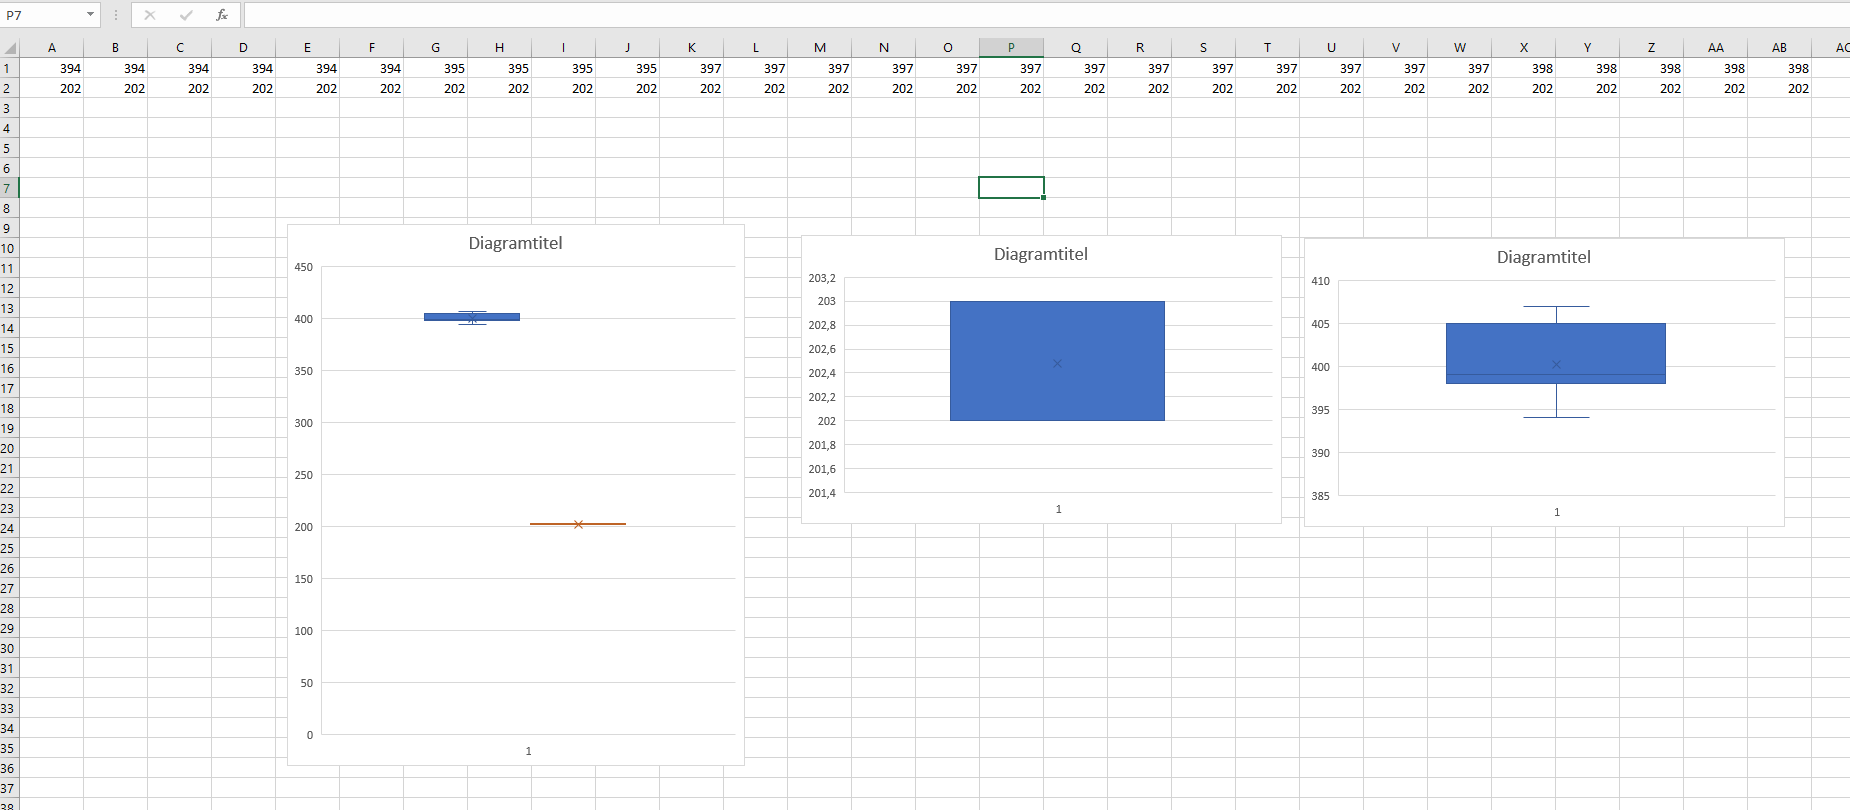
\includegraphics[width=9cm,height=5cm]{box plot.PNG}
\label{fig:cclogo}
\end{center}
\label{fig:firstFigureLabel}
\end{figure}


Vi kan se ud fra vores box plot at vores mean og standard diviacion på ingen måde overlapper og at der tydeligt er et proformance boost i vores program.  \\

\subsection{make the program 50 procent more efficient}


Vi kan se at vores avrage proformance før optimering ligger omkring 400 milisec
og at den ligger omkring 200 efter. Vi har derfor opnået en 50 procent forbedring.



\end{document}
